
%(BEGIN_QUESTION)
% Copyright 2008, Tony R. Kuphaldt, released under the Creative Commons Attribution License (v 1.0)
% This means you may do almost anything with this work of mine, so long as you give me proper credit

This variable-frequency motor drive (VFD) circuit converts three-phase AC power at 60 Hz into rectified and filtered DC, then switches that DC into three-phase AC of whatever frequency desired.  The control circuitry for triggering the MOSFETs is not shown in this diagram, for the sake of simplicity:

$$\includegraphics[width=15.5cm]{i01723x01.eps}$$

Your task is to determine the states (ON or OFF) of those six transistors during each of the time periods shown in the oscillograph:

$$\includegraphics[width=15.5cm]{i01723x02.eps}$$

% No blank lines allowed between lines of an \halign structure!
% I use comments (%) instead, so that TeX doesn't choke.

$$\vbox{\offinterlineskip
\halign{\strut
\vrule \quad\hfil # \ \hfil & 
\vrule \quad\hfil # \ \hfil & 
\vrule \quad\hfil # \ \hfil & 
\vrule \quad\hfil # \ \hfil & 
\vrule \quad\hfil # \ \hfil & 
\vrule \quad\hfil # \ \hfil & 
\vrule \quad\hfil # \ \hfil \vrule \cr
\noalign{\hrule}
%
% First row
Time period & $Q_1$ & $Q_2$ & $Q_3$ & $Q_4$ & $Q_5$ & $Q_6$ \cr
%
\noalign{\hrule}
%
% Another row
$t_1 - t_2$ &  &  &  &  &  & \cr
%
\noalign{\hrule}
%
% Another row
$t_2 - t_3$ &  &  &  &  &  & \cr
%
\noalign{\hrule}
%
% Another row
$t_3 - t_4$ &  &  &  &  &  & \cr
%
\noalign{\hrule}
%
% Another row
$t_4 - t_5$ &  &  &  &  &  & \cr
%
\noalign{\hrule}
%
% Another row
$t_5 - t_6$ &  &  &  &  &  & \cr
%
\noalign{\hrule}
%
% Another row
$t_6 - t_7$ &  &  &  &  &  & \cr
%
\noalign{\hrule}
} % End of \halign 
}$$ % End of \vbox

Assume a ``positive'' current on the graph is one where the drive {\it sources} current to the motor, and a ``negative'' current on the graph is one where the drive {\it sinks} current from the motor.

\vskip 20pt \vbox{\hrule \hbox{\strut \vrule{} {\bf Suggestions for Socratic discussion} \vrule} \hrule}

\begin{itemize}
\item{} What would be different, if anything, about the switching of these six power transistors to make the motor spin {\it faster}?
\item{} What would be different, if anything, about the switching of these six power transistors to make the motor spin in {\it reverse} rather than forward?
\end{itemize}

\underbar{file i01723}
%(END_QUESTION)





%(BEGIN_ANSWER)

% No blank lines allowed between lines of an \halign structure!
% I use comments (%) instead, so that TeX doesn't choke.

$$\vbox{\offinterlineskip
\halign{\strut
\vrule \quad\hfil # \ \hfil & 
\vrule \quad\hfil # \ \hfil & 
\vrule \quad\hfil # \ \hfil & 
\vrule \quad\hfil # \ \hfil & 
\vrule \quad\hfil # \ \hfil & 
\vrule \quad\hfil # \ \hfil & 
\vrule \quad\hfil # \ \hfil \vrule \cr
\noalign{\hrule}
%
% First row
Time period & $Q_1$ & $Q_2$ & $Q_3$ & $Q_4$ & $Q_5$ & $Q_6$ \cr
%
\noalign{\hrule}
%
% Another row
$t_1 - t_2$ & ON & off & off & ON & ON & off \cr
%
\noalign{\hrule}
%
% Another row
$t_2 - t_3$ & off & ON & off & ON & ON & off \cr
%
\noalign{\hrule}
%
% Another row
$t_3 - t_4$ & off & ON & ON & off & ON & off \cr
%
\noalign{\hrule}
%
% Another row
$t_4 - t_5$ & off & ON & ON & off & off & ON \cr
%
\noalign{\hrule}
%
% Another row
$t_5 - t_6$ & ON & off & ON & off & off & ON \cr
%
\noalign{\hrule}
%
% Another row
$t_6 - t_7$ & ON & off & off & ON & off & ON \cr
%
\noalign{\hrule}
} % End of \halign 
}$$ % End of \vbox

If PWM is being used to modulate the output into a quasi-sine wave, then the ``ON'' states shown in the table do not necessarily represent {\it full, continuous on} states within the specified timeframes, but rather series of on/off pulses.  The ``off'' states shown in the table, however, do indeed represent {\it full, continuous off} states within each specified timeframe.

To be more precise in my answer, the table should look like this:

% No blank lines allowed between lines of an \halign structure!
% I use comments (%) instead, so that TeX doesn't choke.

$$\vbox{\offinterlineskip
\halign{\strut
\vrule \quad\hfil # \ \hfil & 
\vrule \quad\hfil # \ \hfil & 
\vrule \quad\hfil # \ \hfil & 
\vrule \quad\hfil # \ \hfil & 
\vrule \quad\hfil # \ \hfil & 
\vrule \quad\hfil # \ \hfil & 
\vrule \quad\hfil # \ \hfil \vrule \cr
\noalign{\hrule}
%
% First row
Time period & $Q_1$ & $Q_2$ & $Q_3$ & $Q_4$ & $Q_5$ & $Q_6$ \cr
%
\noalign{\hrule}
%
% Another row
$t_1 - t_2$ & pulse & off & off & pulse & pulse & off \cr
%
\noalign{\hrule}
%
% Another row
$t_2 - t_3$ & off & pulse & off & pulse & pulse & off \cr
%
\noalign{\hrule}
%
% Another row
$t_3 - t_4$ & off & pulse & pulse & off & pulse & off \cr
%
\noalign{\hrule}
%
% Another row
$t_4 - t_5$ & off & pulse & pulse & off & off & pulse \cr
%
\noalign{\hrule}
%
% Another row
$t_5 - t_6$ & pulse & off & pulse & off & off & pulse \cr
%
\noalign{\hrule}
%
% Another row
$t_6 - t_7$ & pulse & off & off & pulse & off & pulse \cr
%
\noalign{\hrule}
} % End of \halign 
}$$ % End of \vbox

%(END_ANSWER)





%(BEGIN_NOTES)


%INDEX% Final Control Elements, motor: variable frequency drive

%(END_NOTES)


